% Created 2020-12-09 Wed 19:55
% Intended LaTeX compiler: pdflatex
\documentclass{article}
\usepackage[utf8]{inputenc}
\usepackage[T1]{fontenc}
\usepackage{graphicx}
\usepackage{grffile}
\usepackage{longtable}
\usepackage{wrapfig}
\usepackage{rotating}
\usepackage[normalem]{ulem}
\usepackage{amsmath}
\usepackage{textcomp}
\usepackage{amssymb}
\usepackage{capt-of}
\usepackage{hyperref}
\bibliographystyle{plain}}
\usepackage[margin=1.0in]{geometry}
\author{Keagan McMahon, Brigitta Munds, \\ Benjamin Brown, \& Christina Rachmadita}
\date{\textit{<2020-12-14 Mon>} December 14th, 2020}
\title{PSYCH 363 - Stroop Effect: Congruency and Response Time}
\hypersetup{
 pdfauthor={Keagan McMahon, Brigitta Munds, \\ Benjamin Brown, \& Christina Rachmadita},
 pdftitle={PSYCH 363 - Stroop Effect: Congruency and Response Time},
 pdfkeywords={},
 pdfsubject={},
 pdfcreator={Emacs 26.3 (Org mode 9.1.9)}, 
 pdflang={English}}
\begin{document}

\maketitle
\tableofcontents



\section{Introduction}
\label{sec:org72dda60}

\hspace{1em} Previous studies in the Stroop literature have demonstrated that participants might respond differently based on if Stroop items are congruent with their displayed state and some have found evidence of congruency effects \cite{SpinelliGiacomo2020WMLD}. For example, words that are presented in the same colour that the word is describing (i.e. the word "Red" presented in the colour red) would be known as a congruent trial, whereas words presented in a different colour (i.e. "Red, but presented in the colour blue) would be an incongruent trial.\\

Rey-Mermet discusses the idea of attentional-control processes, namely, our ability to ``activate goal-relevant information and to inhibit irrelevant information'' \cite{Mermet2020Faib}. Our study approaches this idea and seeks to understand if reaction time differences arise when comparing congruent to incongruent trials. A participants goal is to correctly report words that are congruent, while inhibiting the irrelevant information presented during incongruent trials and we hypothesize that ones reaction time should differ as a function of the extended cognitive process one must engage in to correctly make this rejection. 

\section{Methods}
\label{sec:org13af32e}

\hspace{1em} \textbf{Participants.} We utilized our 4 group members, and each completed 20 trials 5 times yielding 100 total trials per person. This gave us enough data to be confident in our results, although with such a small sample size of participants it is clear that these results will struggle to generalize to the broader population more broadly. \\

\textbf{Materials.} A program was developed for use in our experiement to randomly choose different colour words (i.e. red, blue, green, etc) and an associated colour that the words were written in. The words are presented on a plain solid grey background and participants were instructed to either press "z" or "/" on a keyboard to indicate whether the word and its associated colour were congruent (i.e. the written word matched the colour of the word) or incongruent (i.e. the written word did not match the colour of the word). After each user response a new word would be randomly generated for them to respond to and once the participant completes 20 trials, the program closes itself, the data is exported and procedure ends. Importantly, the colour and word displayed were all randomly selected, the probability of a participant seeing a congruent trial was set at 25\%. \\

Please see below for a copy of the Python code used in designing the program: \\
\begin{verbatim}
from psychopy import visual,core,clock,event
import random as r
import csv
from datetime import datetime

now=datetime.now()
date_time=now.strftime("%Y-%m-%d_%H:%M:%S")
filename="stroop"+date_time+".csv"

keyAssign=["q","z","slash"]
colourOptions=["yellow","red","blue","green"]

probCongruent=0.25

numberTrials=20
RTclock=core.Clock()

win=visual.Window(size=(600,600))

instructionText="Press 'z' for congruent words & colours  and '/' when incongruent. 
Press any key to start."

showInstruction=visual.TextStim(win,instructionText,color="black",height=0.1)
showInstruction.draw()
win.flip()
event.waitKeys()

for i in range(numberTrials):

	r.shuffle(colourOptions)

	if r.random()<probCongruent:
		writtenColour=colourOptions[0]
		displayColour=colourOptions[0]
		congruent=1
	else:
		writtenColour=colourOptions[0]
		displayColour=colourOptions[1]
		congruent=0


	displayText = visual.TextStim(win,writtenColour,color=displayColour,height=0.2)

	displayText.draw()
	win.flip()
	RTclock.reset()
	key=event.waitKeys(keyList=keyAssign)
	rt=RTclock.getTime()
	if (key[0]==keyAssign[0]):
		core.quit()

	with open(filename,'a',newline='') as csvfile:
		posnerwrite=csv.writer(csvfile,delimiter=' ')
		posnerwrite.writerow([writtenColour] + [displayColour] + [congruent] + [key[0]] + [rt])

core.wait(1)
core.quit()
\end{verbatim}
\section{Results}
\label{sec:org7cf09a1}

\begin{verbatim}

## Read participant data file
dt <- read.csv("363Stroop_Data_Dec_4.csv")

\end{verbatim}

\textbf{Data structure:} This produces an example excerpt from our CSV file (up to 10 trials), there are 400 total across the entire experiment. As you can see, the data is automaticallly arranged based on if the trial is congruent or not (1 for congruent, 0 for incongruent), the presented colour, the participants response, and their reaction time.
\begin{verbatim}

## An example of how our data is structured
head(dt, 10)
\end{verbatim}

\begin{verbatim}
   Trial Congruent Colour Response      Time
1      1         1   blue        z 1.0113984
2      1         0   blue    slash 0.9906640
3      1         0    red    slash 0.7729855
4      1         0  green    slash 0.7496739
5      1         0  green    slash 0.6566195
6      1         1 yellow        z 0.5783305
7      1         0  green    slash 1.0228071
8      1         0  green    slash 1.3865062
9      1         0 yellow    slash 0.7888217
10     1         0   blue    slash 0.9663929
\end{verbatim}

\vspace{2em} \textbf{Statistical Summary of the Data:} This produces some basic descriptive statistics of our experiment. To note a few, there were 88 trials were participants hit the 'z' key (i.e. reported a congruent trial) and 312 instances where they hit the '/' key (i.e. reported an incongruent trial). The mean response time was 0.8997 seconds with the longest response taking 4.5227 seconds and the quickest response taking 0.2039 seconds. 
\begin{verbatim}

summary(dt)

\end{verbatim}

\begin{verbatim}
    Trial         Congruent         Colour     Response        Time       
Min.   : 1.00   Min.   :0.0000   blue  :110   slash:312   Min.   :0.2039  
1st Qu.: 5.75   1st Qu.:0.0000   green : 82   z    : 88   1st Qu.:0.6608  
Median :10.50   Median :0.0000   red   :102               Median :0.7536  
Mean   :10.50   Mean   :0.2175   yellow:106               Mean   :0.8997  
3rd Qu.:15.25   3rd Qu.:0.0000                            3rd Qu.:0.9482  
Max.   :20.00   Max.   :1.0000                            Max.   :4.5227
\end{verbatim}

\textbf{Number of rows/trials}: This displays the total number of rows in our data file, equivalent to the total number of trials within our experiment.
\begin{verbatim}
nrow(dt)
\end{verbatim}

\begin{verbatim}
[1] 400
\end{verbatim}


\vspace{2em} \textbf{Linear Regression Model:} We completed many different statistical analyses on our data, the first being a linear regression. Our results show that <1\% of the total variation in participant response times can be explained by our independent variable, congruency. 
\begin{verbatim}
lmresults <- lm( Time ~ Congruent, data = dt)
summary(lmresults)
\end{verbatim}

\begin{verbatim}

Call:
lm(formula = Time ~ Congruent, data = dt)

Residuals:
    Min      1Q  Median      3Q     Max 
-0.7115 -0.2423 -0.1421  0.0377  3.6073 

Coefficients:
            Estimate Std. Error t value Pr(>|t|)    
(Intercept)  0.91539    0.02736  33.456   <2e-16 ***
Congruent   -0.07234    0.05867  -1.233    0.218    
---
Signif. codes:  0 ‘***’ 0.001 ‘**’ 0.01 ‘*’ 0.05 ‘.’ 0.1 ‘ ’ 1

Residual standard error: 0.4841 on 398 degrees of freedom
Multiple R-squared:  0.003806,	Adjusted R-squared:  0.001303 
F-statistic:  1.52 on 1 and 398 DF,  p-value: 0.2183
\end{verbatim}

\vspace{2em} \textbf{Specialised T-test:} The second test we ran was a Welch Two Sample T-test and as we can see from our results that there is not enough evidence to suggest that reaction times are significantly different when presented congruent trials than when presented incongruent trials and we must retain the null hypothesis, t(241) = 1.646, p > .05.
\begin{verbatim}
t.test(Time ~ Congruent, mu=0, alt="two.sided", conf=0.95, var.eq=F, paired=F, data = dt)
\end{verbatim}

\begin{verbatim}

	Welch Two Sample t-test

data:  Time by Congruent
t = 1.6466, df = 241.61, p-value = 0.1009
alternative hypothesis: true difference in means is not equal to 0
95 percent confidence interval:
 -0.01420303  0.15888674
sample estimates:
mean in group 0 mean in group 1 
      0.9153860       0.8430441
\end{verbatim}

\vspace{11em} \textbf{One-Way ANOVA:} The third test we ran was a One-Way Analysis of Variance and like the other tests our results do not provide sufficient evidence that reaction times differ significantly under different levels of congruency, F(1, 398) = 1.52, MSE = 0.35, p > .05.
\begin{verbatim}
anova(lmresults)
\end{verbatim}

\begin{verbatim}
Analysis of Variance Table

Response: Time
           Df Sum Sq Mean Sq F value Pr(>F)
Congruent   1  0.356 0.35627  1.5205 0.2183
Residuals 398 93.258 0.23432
\end{verbatim}

\vspace{2em} \textbf{More Linear Regression:} We decided to further explore the explanatory power between the other variables as well\ldots{} this really isn't relevant, delete? explanatory power of trial \#, response, and colour value? Marked for removal.
\begin{verbatim}
lmresults2 <- lm( Time ~ Congruent + Trial + Colour + Response, data = dt)
summary(lmresults2)
\end{verbatim}

\begin{verbatim}

Call:
lm(formula = Time ~ Congruent + Trial + Colour + Response, data = dt)

Residuals:
    Min      1Q  Median      3Q     Max 
-0.5683 -0.2452 -0.1264  0.0476  3.5778 

Coefficients:
              Estimate Std. Error t value Pr(>|t|)    
(Intercept)   0.985707   0.067434  14.617   <2e-16 ***
Congruent     0.727180   0.488648   1.488    0.138    
Trial        -0.006801   0.004213  -1.614    0.107    
Colourgreen   0.065221   0.070966   0.919    0.359    
Colourred    -0.045419   0.066993  -0.678    0.498    
Colouryellow  0.004813   0.065793   0.073    0.942    
Responsez    -0.799422   0.486281  -1.644    0.101    
---
Signif. codes:  0 ‘***’ 0.001 ‘**’ 0.01 ‘*’ 0.05 ‘.’ 0.1 ‘ ’ 1

Residual standard error: 0.4829 on 393 degrees of freedom
Multiple R-squared:  0.02085,	Adjusted R-squared:  0.005901 
F-statistic: 1.395 on 6 and 393 DF,  p-value: 0.2154
\end{verbatim}

\vspace{2em} \textbf{One-Way ANOVA (again? what is this for?):} \^{}\^{}\^{} see more linear regression comment, same thing but an anova. Marked for removal, not relevant. 
\begin{verbatim}
anova(lmresults2)
\end{verbatim}

\begin{verbatim}
Analysis of Variance Table

Response: Time
           Df Sum Sq Mean Sq F value Pr(>F)
Congruent   1  0.356 0.35627  1.5275 0.2172
Trial       1  0.505 0.50535  2.1667 0.1418
Colour      3  0.460 0.15330  0.6573 0.5788
Response    1  0.630 0.63034  2.7026 0.1010
Residuals 393 91.662 0.23324
\end{verbatim}

\subsection{Plots}
\label{sec:org392119a}
\subsubsection{Mean Reaction Time: Congruent vs Incongruent Trials}
\label{sec:orge3d03ca}
\begin{verbatim}

p <- ggplot(overall, aes(x = cond, y = rt)) + geom_bar(fill = "darkturquoise", stat = "identity", 
width = 0.5) + labs(title = "Mean Reaction Time", x = "Condition", 
y = "Reaction Time (seconds)") + theme_classic() + 
theme(plot.title = element_text(hjust = 0.5, size = 15, face = "bold"), 
panel.background = element_blank(), panel.grid = element_blank(), 
panel.border = element_rect(colour = "black", fill = NA, size = 0.75))

p
\end{verbatim}

\begin{center}

\includegraphics[width=.9\linewidth]{converted_stroop2.png}
\end{center}

\subsubsection{RT Values for Congruent Trials}
\label{sec:org8a70b06}
\begin{verbatim}

RT_congruent <- ggplot(df, aes(x = Congruent)) + geom_histogram(alpha = 0.5, fill = "steelblue", 
color = "white") + labs(title = "Response Time for Congruent Words", x = "Response Time (seconds)", 
y = "Frequency") + theme_classic() + theme(plot.title = element_text(hjust = 0.5, size = 15, 
face = "bold"), panel.background = element_blank(), panel.grid = element_blank(), 
panel.border = element_rect(colour = "black", 
fill = NA, size = 0.75)) + xlim(0.25, 1.75) + ylim(0, 5)

RT_congruent

\end{verbatim}

\begin{center}
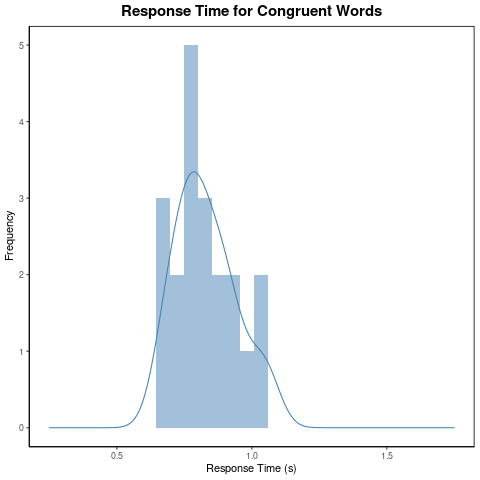
\includegraphics[width=.9\linewidth]{converted_stroop5.png}
\end{center}

\subsubsection{RT Values for Incongruent Trials}
\label{sec:org5086791}
\begin{verbatim}

RT_incongruent <- ggplot(df, aes(x = Incongruent)) + geom_histogram(alpha = 0.5, fill = "steelblue", 
color = "white") + labs(title = "Response Time for Incongruent Words", x = "Response Time (seconds)", 
y = "Frequency") + theme_classic() + theme(plot.title = element_text(hjust = 0.5, size = 15, 
face = "bold"), panel.background = element_blank(), panel.grid = element_blank(), 
panel.border = element_rect(colour = "black", 
fill = NA, size = 0.75)) + xlim(0.25, 1.75) + ylim(0, 5)

RT_incongruent

\end{verbatim}

\begin{center}
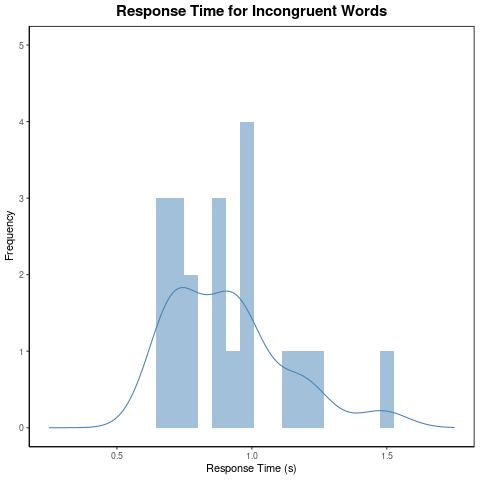
\includegraphics[width=.9\linewidth]{converted_stroop6.png}
\end{center}

\subsubsection{Response Time Density Plot}
\label{sec:orgfb08943}
\begin{verbatim}

density_plot <- ggplot(cond_rt_df, aes(x = RT, color = Condition, fill = Condition)) + 
geom_density(alpha = 0.5) + labs(title = "Response Time Density Plot", x = "Response Time (seconds)", 
y = "Frequency") + theme_classic() + theme(plot.title = element_text(hjust = 0.5, size = 15, 
face = "bold"), legend.position = "right", legend.background = element_blank(), 
legend.box.background = element_rect(colour = "black"), panel.background = element_blank(), 
panel.grid = element_blank(), panel.border = element_rect(colour = "black", 
fill = NA, size = 0.75)) + xlim(0.25, 1.75) 

density_plot

\end{verbatim}

\begin{center}

\includegraphics[width=.9\linewidth]{converted_stroop3.png}
\end{center}


\section{Discussion}
\label{sec:org696bea0}

\hspace{1em} Our study originally hypothesized that there should be a difference in participant reaction time due to the increased cognitive effort one must expend to inhibit irrelevant information (i.e. in this case, incongruent trials) when compared to trials where they presumably would have to expend less effort (i.e. during congruent trials). We believed therefore that incongruent trials should lead to participants taking longer to complete and congruent trials should be relatively quicker due to one not having to bypass the barrier of the required extra processing to make a correct rejection on false targets (i.e. incongruent trials). Spinelli and Lupker found in a 2020 study a significant result indicating faster response times for congruent trials than incongruent trials \cite{SpinelliGiacomo2020I}. Our study finds quite the opposite and we believe this opens up the body of research for continued study and investigation. However, there are some glaringly clear limitations to our study and earlier attempts at these studies as we have seen from Spinelli and the like should not be discarded. Firstly, our study had an extremely small sample size of only 4 participants, all of which had a hand in deciding the study and this could negatively bias our results. By proxy we had a very small set of trials, 400 is acceptable with 100 per person, but given that there were again only 4 people this is a clear limitation. Lastly, our study was not conducted in a controlled lab setting and this could skew our results as a consequence. 

\bibliography{stroopBib.bib}
\end{document}
